\section{Kiến trúc Hệ thống \& Cấu trúc Tô-pô Mạng}

\subsection{Phân tầng Kiến trúc OpenStack}
Hệ thống OpenStack vận hành theo mô hình kiến trúc phân tán dạng hướng dịch vụ (Microservices), trong đó các dịch vụ độc lập giao tiếp với nhau thông qua giao diện lập trình ứng dụng RESTful HTTP APIs và hàng đợi thông điệp RabbitMQ, dưới sự chứng thực tập trung của dịch vụ định danh Keystone~\cite{openstack_arch, devstack_docs} (Hình~\ref{fig:sys_architecture}).

\begin{figure}[H]
\centering
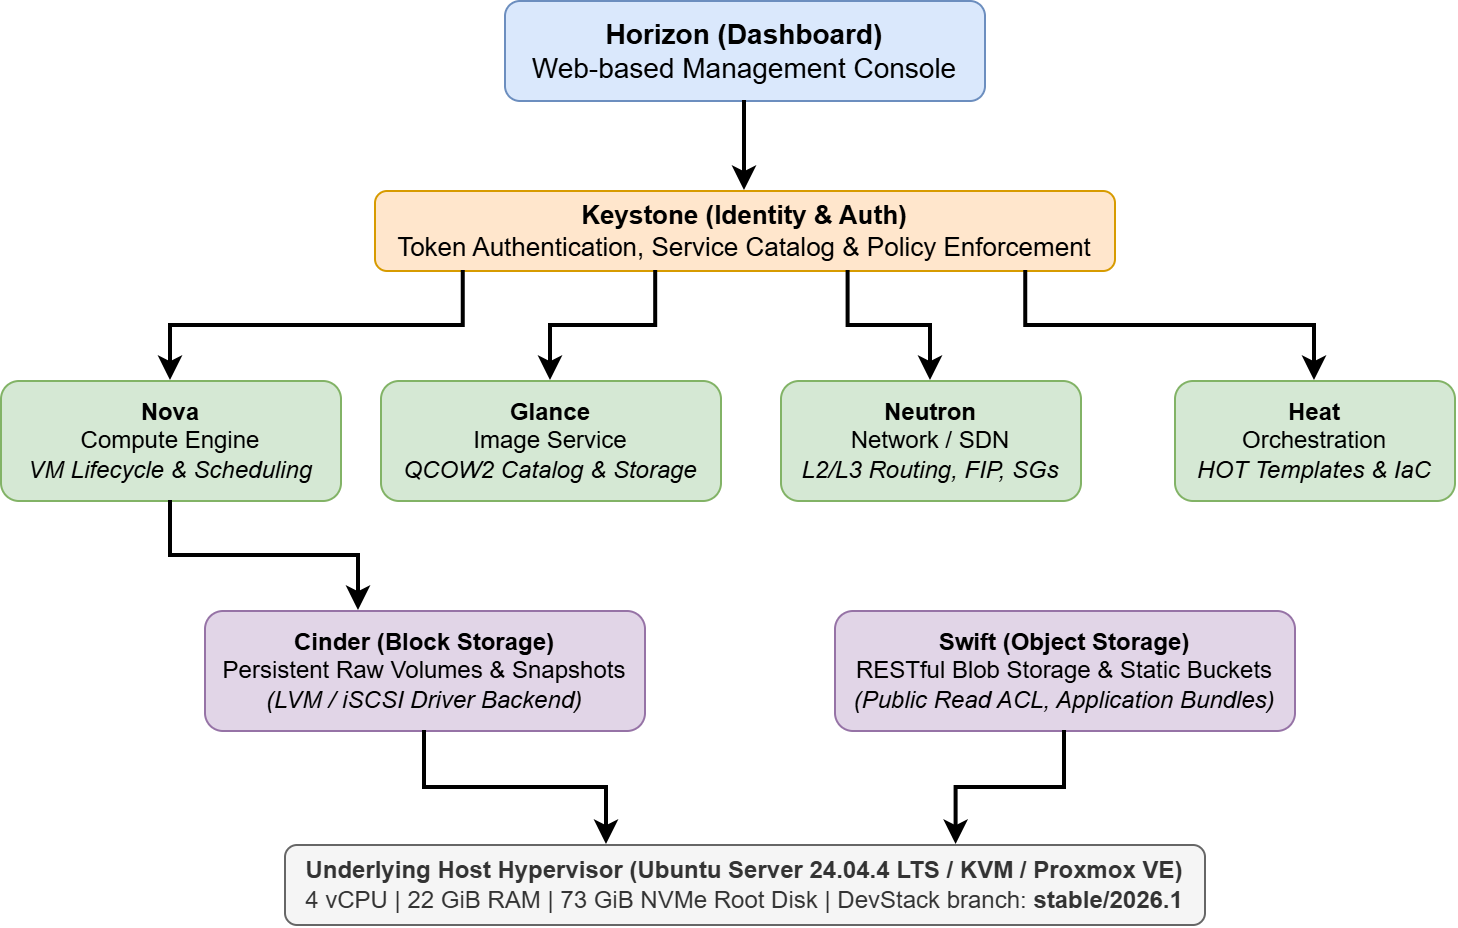
\includegraphics[width=0.92\linewidth]{img/openstack_architecture.png}
\caption{Kiến trúc phân tầng và luồng tương tác giữa các vi dịch vụ trong hệ thống OpenStack.}
\label{fig:sys_architecture}
\end{figure}

Trong phạm vi triển khai của đồ án, các khối dịch vụ cốt lõi đảm nhận các vai trò kỹ thuật cụ thể như sau:
\begin{enumerate}
    \item \textbf{Xác thực \& Định danh (Keystone):} Xác thực các yêu cầu API, phát hành mã token có phạm vi truy cập (Scoped Token) và phân giải URL endpoint của các dịch vụ trong mạng nội bộ cũng như mạng quản trị.
    \item \textbf{Quản lý Điện toán (Nova):} Tương tác với hệ thống quản lý ảo hóa \texttt{libvirt/qemu} để quản lý vòng đời máy ảo, lập lịch thực thi trên hypervisor và cấp phát đĩa gốc (Ephemeral Root Disk).
    \item \textbf{Quản lý Ảnh máy ảo (Glance):} Lưu trữ và phân phối các tệp ảnh hệ điều hành tương thích với Cloud-Init (\texttt{cirros-0.6.3-x86\_64-disk} và \texttt{Fedora-Cloud-Base-37-1.7}).
    \item \textbf{Mạng ảo hóa phần mềm (Neutron):} Quản lý hạ tầng mạng ảo SDN~\cite{neutron_guide}, các phân đoạn mạng tenant, bộ định tuyến ảo L3 Router và tường lửa phân tán (Security Groups).
    \item \textbf{Hệ thống Lưu trữ (Cinder \& Swift):}
    \begin{itemize}
        \item \textbf{Cinder~\cite{cinder_storage}:} Cung cấp các khối lưu trữ bền vững (Block Storage) gắn vào máy ảo qua giao thức iSCSI/LVM.
        \item \textbf{Swift~\cite{swift_storage}:} Cung cấp dịch vụ lưu trữ đối tượng (Object Storage) chuẩn REST API phục vụ lưu trữ file tĩnh và mã nguồn ứng dụng.
    \end{itemize}
    \item \textbf{Tự động hóa Điều phối (Heat):} Phân tích cú pháp các tệp mẫu khai báo YAML (HOT specification)~\cite{heat_hot_guide}, xây dựng đồ thị có hướng không chu trình (DAG) để tự động khởi tạo hạ tầng theo đúng thứ tự phụ thuộc.
\end{enumerate}

\subsection{Kiến trúc Mạng Phân tầng (Multi-Tier Topology)}
Hình~\ref{fig:net_architecture} thể hiện sơ đồ tô-pô mạng logic mà nhóm chúng em đã thiết kế và triển khai xuyên suốt từ Module 2 đến Module 4, mô phỏng cấu trúc mạng phân tầng bảo mật cho doanh nghiệp tuân thủ theo chuẩn RFC 1918~\cite{rfc1918}.

\begin{figure}[H]
\centering
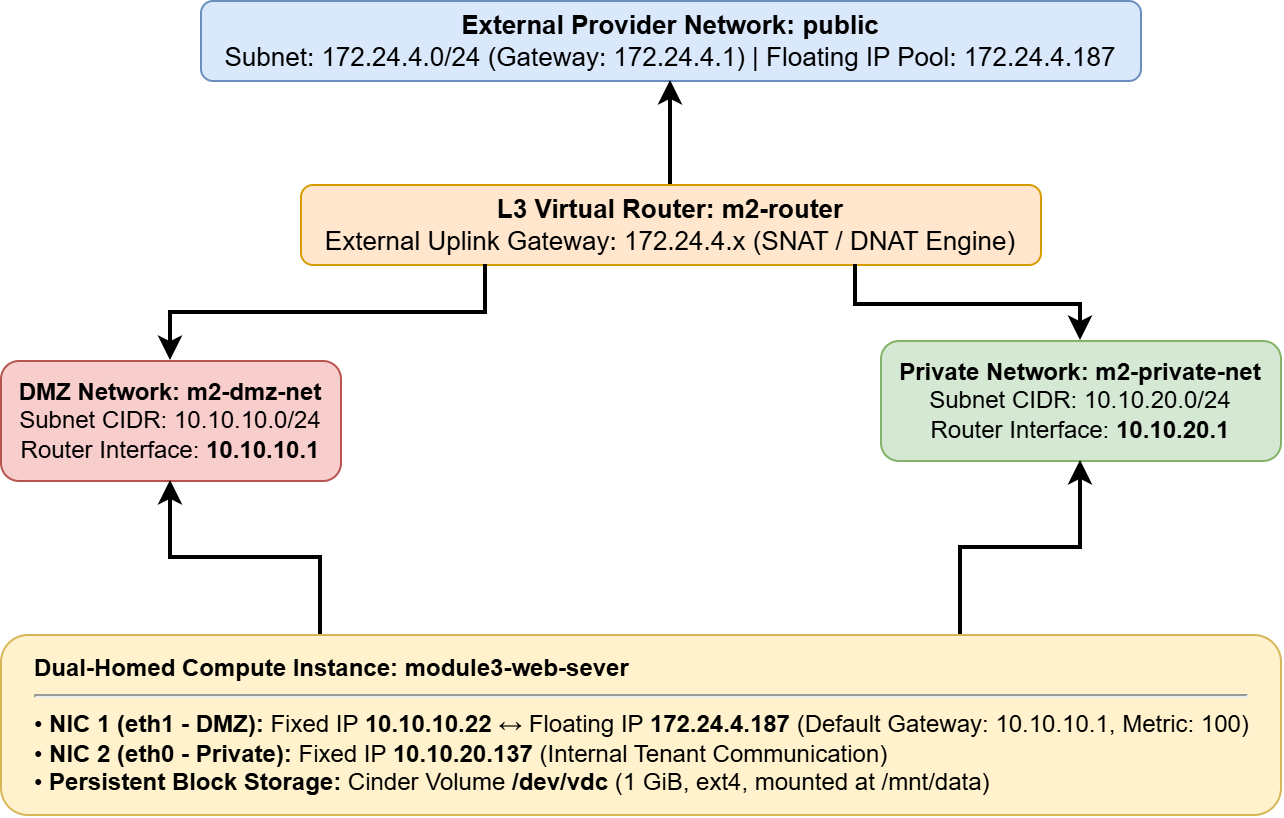
\includegraphics[width=0.92\linewidth]{img/network_topology.png}
\caption{Tô-pô mạng logic thể hiện sự cô lập đa tầng, định tuyến L3 và kết nối máy ảo đa card mạng.}
\label{fig:net_architecture}
\end{figure}
